\documentclass[runningheads,a4paper]{llncs}
\bibliographystyle{ieeetr}
\usepackage{graphicx}
% 
\usepackage{mathabx}
\usepackage{array}
\usepackage{hyperref}
\usepackage{indentfirst}
\usepackage{subcaption}
\usepackage{todonotes}
\newenvironment{frcseries}{\fontfamily{frc}\selectfont}{}
\newcommand{\textfrc}[1]{{\frcseries#1}}
\usepackage{array,multirow,makecell}
\setcellgapes{1pt}
\makegapedcells
\newcolumntype{R}[1]{>{\raggedleft\arraybackslash }b{#1}}
\newcolumntype{L}[1]{>{\raggedright\arraybackslash }b{#1}}
\newcolumntype{C}[1]{>{\centering\arraybackslash }b{#1}}
\usepackage{booktabs}
\usepackage{multirow}
\usepackage{siunitx}
\newcommand{\argmax}[1]{\underset{#1}{\operatorname{arg}\,\operatorname{max}}\;}
\usepackage{algorithm,algorithmic}
\usepackage{float}
\usepackage{comment}
\usepackage{lipsum}
\usepackage{csvsimple}
\usepackage{xstring}  

\makeatletter
\newcommand\footnoteref[1]{\protected@xdef\@thefnmark{\ref{#1}}\@footnotemark}
\makeatother

\makeatletter
\csvset{
  autotabularleft/.style={
    file=#1,
    after head=\csv@pretable\begin{tabular}{|l|*{\csv@columncount}{r|}}\csv@tablehead,
    table head=\hline\csvlinetotablerow\\\hline,
    late after line=\IfBeginWith{\csvcoli}{-}{\\}{\\\hline},
    table foot=\\\hline,
    late after last line=\csv@tablefoot\end{tabular}\csv@posttable,
    command=\csvlinetotablerow},
}
\makeatother
\newcommand{\csvautotabularleft}[2][]{\csvloop{autotabularleft={#2},#1}}

\title{DOREMUS: A Graph of Linked Musical Works}

\titlerunning{}


%\titlerunning{}

\author{Manel Achichi,$^1$  Pasquale Lisena,$^2$   Konstantin Todorov,$^{1}$  Rapha\"el Troncy,$^2$ Jean Delahousse$^3$}
\authorrunning{Achichi, Lisena, Todorov, Troncy, Delahousse}

\institute{
LIRMM, University of Montpellier, CNRS, France \\ \{\textbf{achichi, todorov}\}\textbf{@lirmm.fr}
\and
EURECOM, Sophia Antipolis, France \\ \{\textbf{pasquale.lisena, raphael.troncy}\}\textbf{@eurecom.fr}
\and
OUROUK, Paris, France \\ \textbf{delahousse.jean}\textbf{@gmail.com}}

\begin{document}

\maketitle

\begin{abstract} 
Three major French cultural institutions---the French National Library (BnF), Radio France and the Philharmonie de Paris---have come together in order to develop shared methods to describe semantically their catalogs of music works and events. This process comprises the construction of knowledge graphs representing the data contained in these catalogs following a novel agreed upon ontology that extends CIDOC-CRM and FRBRoo, the linking of these graphs and their open publication on the web. A number of specialized tools  that allow for the reproduction of this process are developed, as well as web applications for easy access and navigation through the data. The paper presents one of the main outcomes of this project---the DOREMUS knowledge graph, consisting of three linked datasets describing classical music works and their associated events (e.g., performances in concerts). This resource fills an important gap between library content description and music metadata. We present the DOREMUS pipeline for lifting and linking the data, the tools developed for these purposes, as well as a search application allowing to explore the data.
\end{abstract}

\section{Introduction} \label{sec:intro}
The Linked Open Data (LOD) paradigm for data representation, sharing and publishing has been more and more appealing to the world of museums and libraries over the past years. The LOD project and the semantic web in general offer technological means for data reuse, increased visibility and data sharing on the web, data federation and facilitated exchange of metadata by the creation of links across resources. Attracted by these possibilities, many major actors from the library world, such as the Library of Congress (LOC) or the French National Library (BnF), have embraced semantic web technologies with the goal to open their archives and catalogs to the web. This process has resulted in a number of openly available and explorable RDF graphs reflecting the rich content of numerous libraries and cultural institutions from all over the world~\cite{marden2013linked}.

The DOREMUS project follows this line of research and practice, with a particular interest in classical and traditional music, so far relatively underrepresented on the LOD.\footnote{\url{http://www.doremus.org}} Three major French cultural institutions---the BnF, Radio France (RF) and the Philharmonie de Paris (PP)---have joint efforts with data and social science academics in order to develop shared methods to describe semantically their catalogs of music works and events and open them to the web community. A major contribution of the project is the development of the DOREMUS ontology\footnote{\url{http://data.doremus.org/ontology/}} which extends the well-known CIDOC-CRM and FRBRoo models for representing bibliographic information\footnote{\url{http://new.cidoc-crm.org/frbroo/}}, adapting it to the domain of music, thus filling an important representational gap. A number of shared vocabularies about music-specific concepts (such as musical genres or keys) have been collected or developed, linked and published using the SKOS standard. The data from the catalogs of the three partner institutions comes in MARC or XML  formats. Specific tools for data conversion to RDF following the DOREMUS model have been developed. This process results in the construction of several knowledge graphs about music works and events, which have been linked using a specifically developed for this purpose data linking tool. For evaluation purposes, a benchmark has been created manually by the library experts and shared to the semantic web community as part of the Ontology Alignment Evaluation Initiative (OAEI). The data fusion process results in the construction of a pivot graph of shared and unique musical works. Finally, an exploratory search engine is developed that allows to browse the knowledge graphs.

This paper covers the components of the DOREMUS workflow described above, which altogether form a paradigm for lifting, linking and publishing music library metadata. We present in detail the DOREMUS knowledge graphs with a focus on the (re-)used models and vocabularies and the processes that allow for their (re-)production and fusion. The contributions of this work are:

$\bullet$ A model for describing musical works and events extending FRBRoo together with a number of shared and linked music-specific controlled vocabularies.

$\bullet$ Three knowledge graphs about music works that represent the catalogs of three major French cultural institutions.

$\bullet$ An approach to interlink these graphs resulting in the construction of a pivot graph, containing all unique works and links to the original graphs. 

$\bullet$ A set of benchmark datasets for data linking evaluation.

$\bullet$ A set of tools for data generation, vocabulary alignment and validation, data linking, pivot graph construction, and data search and exploration.

The remainder of the paper is structured as follows. In the next section, we provide general information about the graphs, their form and content, the (re-) used ontologies and controlled vocabularies, as well as statistics. In Section~\ref{sec:develop}, we detail the different components of the DOREMUS data production pipeline, and in particular, the data conversion and linking approaches. In Section~\ref{sec:use}, we demonstrate how this resource has already been used and we discuss its wider expected impact. We present related initiatives in Section~\ref{sec:relwork} before we conclude and discuss future work in Section \ref{sec:conclusion}.
\section{The DOREMUS Datasets of Linked Musical Works} \label{sec:doremus}
The DOREMUS knowledge graph consists of several datasets, each  containing the information coming from a specific database of an institution. In that, a given real-world entity (e.g., a music work) is represented at most once in each graph. %As a consequence, \textit{intra}-dataset linking is not needed, while \textit{inter}-dataset linking is required. 
Currently, three stable datasets have been published: {\bf (1)} \texttt{bnf}: Works and Artists, originally described in MARC records of the BnF; {\bf (2)} \texttt{philharmonie}: Works and Concerts, originally described in MARC records of the PP; {\bf (3)} \texttt{itema3}: Concerts and Recordings, originally described in XML records of RF. Each dataset has two access points: (1) A specific named graph in the DOREMUS triplestore, accessible through a public SPARQL endpoint. Each graph follows the pattern \url{http://data.doremus.org/<dataset_name>}. (2) A set of RDF files in Turtle format, available to public download. All datasets are licensed for free distribution, following a Creative Commons Attribution 4.0 license\footnote{\url{https://creativecommons.org/licenses/by/4.0/}} and have a DCAT description in the triplestore itself. All links to DOREMUS datasets or tools are given in Table~\ref{tab:links}. \begin{table}[htbp]
\begin{center} \scriptsize
\begin{tabular}{ll}
{\bf Name of resource or tool and description,  URL } \\ %\hline
 {\bf Data}   \\ %\hline
{\tt bnf}: Works and Artists from the BnF,   \url{http://data.doremus.org/bnf}  \\ 
{\tt philharmonie}: Works and Concerts from the PP,  \url{http://data.doremus.org/philharmonie}  \\ 
{\tt itema3}: Concerts and Recordings from RF,  \url{http://data.doremus.org/itema3}  \\ DOREMUS triplestore,  \url{https://github.com/DOREMUS-ANR/knowledge-base/tree/master/data}  \\ 
DOREMUS sparql endpoint,   \url{http://data.doremus.org/sparql}  \\ 
Example queries,  \url{http://data.doremus.org/queries.html}  \\ 
DOREMUS ontology,   \url{http://data.doremus.org/ontology}  \\
DOREMUS vocabularies,  \url{https://github.com/DOREMUS-ANR/knowledge-base/tree/master/vocabularies}  \\ 
Vocab. Alignments,  \url{https://github.com/DOREMUS-ANR/knowledge-base/tree/master/vocabularies/alignments}  \\ 
DOREMUS linked data, \url{https://github.com/DOREMUS-ANR/knowledge-base/tree/master/linked-data}  \\ 
DOREMUS benchmarks 2016, \url{http://islab.di.unimi.it/content/im_oaei/2016/#doremus} \\
DOREMUS benchmarks 2017,  \url{http://islab.di.unimi.it/content/im_oaei/2017/#doremus} \\
{\bf Tools}   \\ %\hline
{\tt marc2rdf} converter,  \url{https://github.com/DOREMUS-ANR/marc2rdf}  \\ 
{\tt itema3} converter,  \url{https://github.com/DOREMUS-ANR/itema3converter}  \\ 
{\tt euterpe} converter,  \url{https://github.com/DOREMUS-ANR/euterpe-converter}  \\ 
{\it Legato}: instance matcher,  \url{https://github.com/DOREMUS-ANR/legato}  \\ 
DOREMUS pivot graph constructor,  \url{https://github.com/DOREMUS-ANR/pivot-graph-constructor}  \\ 
{\sc Overture} search engine,  \url{http://overture.doremus.org}  \\
YAM++ vocabulary mapping and validation,  \url{http://yamplusplus.lirmm.fr}  \\ 
Learning materials, \url{https://github.com/DOREMUS-ANR/training}  \\ 
% \hline
\end{tabular}
\smallskip
\captionof{table}{Links to DOREMUS resources and tools.}
\label{tab:links}
\end{center}
\end{table}
\vspace{-1.5cm}
\subsection{Content and Form of the Resource}
The DOREMUS knowledge graphs contain information about works (referred to as {\it expressions}) and related entities from the field of classical and traditional music. Each entity is identified by an univocal persistent URI, which follows the pattern \texttt{http://data.doremus.org/<group>/<uuid>}, where the group is determined by the class of the entity (e.g. \texttt{expression}) and the UUID (Universal Unique Identifier) is generated at conversion time in a deterministic way using the dataset name, the class and the identifier of the source record as seed.\footnote{\url{https://github.com/DOREMUS-ANR/marc2rdf/blob/master/URI.patterns.md}} Currently, the resource is shaped by three knowledge graphs of music works (one per institution), that are linked together in a pivot graph, which is the union of all unique expressions across the three bases, together with {\tt owl:sameAs} links to the original graphs (cf. Section \ref{sec:develop}). We find information pertaining to the instruments, genre and key of a music work (e.g., ``piano", ``sonata", ``A-flat major"), its composer and title(s), date of creation, catalog numbers, opus numbers, etc. As an example, we can find all this information linked to \url{http://data.doremus.org/expression/d72301f0-0aba-3ba6-93e5-c4efbee9c6ea}, representing \\Beethoven's \textit{Moonlight Sonata}. Jazz music would contain a different kind of information, as in \url{http://data.doremus.org/expression/cc7fc9a6-124d-3cc1-\\95e7-5644ecb394a6}, representing Coltrane's {\it Naima}.%\footnote{World music will be exposed after conversion.} 

\subsection{(Re-)used Ontologies and Vocabularies} 
The DOREMUS model is an ontology for the description of music catalogs. It is an extension for the music domain of the FRBRoo model for describing librarian information, which has in turn been born as a dialog of the librarian FRBR model and the CIDOC-CRM ontology for representing museum information, putting togheter the distinction between Work, Expression, Manifestation, Item of the former with the centrality of creation events for describing the cultural object lifecycle coming from the latter~\cite{doerr2008frbroo}. On top of the FRBRoo original classes and properties, specific ones have been added in order to describe aspects of a work that are related to music, such as the musical key, the genre, the tempo, the medium of performance (MoP), etc.~\cite{choffe2016doremus}. The model is ready to be used for describing the interconnection of different arts: it is the case of the soundtrack of a movie, or a song that uses the text of a poem.

DOREMUS imports the Work-Expression-Event triplet\footnote{Not to be confused with an RDF triple.} pattern of FRBRoo: the abstract intention of the author (Work) exists only through an Event (i.e. the composition) that realizes it in a distinct series of choices called Expression(s). This pattern ensures that each step of the life of a musical work can be modeled separately, following the same triplet structure. Thinking about a classic work, we will have a triplet for the composition, one for any performance event, one for every manifestation (e.g., the score), all connected in the graph. This means also that each part of the music production process is considered as an Event that gives birth to a new Work and a new Expression: this leads to the creation of classes like Performance Work or Recording Expression. Each triplet contains information that at the same time can live autonomously and be linked to the other entities. This provides the freedom of representing, for example, a jazz improvisation as extemporaneous performance not connected to a particular pre-existing work, or to collect all the recordings of a piece of world music. The result is a model, which is quite complex and hard to adopt if we look at the levels of distribution of information: from an Expression, one has to pass through Event and Activity to reach a composer, or through Casting and Casting detail to get the MoP. On the other hand, the model has a very detailed expressiveness that allows, for instance, to describe different kinds of contributors (not only authors or performers), to detail the casting of a composition (with number, roles, notes for each instrument/voice), to specify performers at level of single performance inside a whole concert. As an extension of FRBRoo, the model appears familiar to librarian catalogers (documentation: \url{http://data.doremus.org/ontology}).

For the description of music-specific concepts like the  key, the genre or the MoP, we publish controlled vocabularies (using SKOS and MODS standards), realized and enriched by an editorial process that involved also librarians, in order to overcome multilingualism and alternative names issues. Some of these vocabularies were already available and in use by the community: in this case our contribution consists in their collection, conversion to SKOS (if needed) and alignment. As a result, we collected, implemented and published 17 controlled vocabularies belonging to 7 different categories (musical keys, types of derivation, modes, thematic catalogs, functions, musical genres and MoP) (Table \ref{tab:links}) \cite{lisena2018vocabularies}. The vocabularies are all available in the DOREMUS triplestore server via its public SPARQL endpoint. Alternatively, they can be explored by a web browser starting from \url{http://data.doremus.org/vocabularies/}. Each vocabulary is licensed for free distribution, following a Creative Commons Attribution 4.0 license. 


The categories of genres and MoPs contain each 6 different vocabularies, including well-established reference thesauri, as well as institution-specific lists. The vocabularies of these two categories have been aligned by establishing {\tt skos:\\exactMatch} relations between their elements in a pairwise manner using an automatic ontology and thesaurus matching system and these alignments have been manually validated and enriched by the experts of the three institutions. This process has been assisted by a dedicated generic web-application for ontology matching and mapping validation, YAM++ {\it online} \cite{bellahsene2017yam++}, developed in part for the purposes of the project (link available in Table \ref{tab:links}).

% The following list reports the vocabularies that we have so far with the number of concepts in parenthesis:
% \begin{enumerate}
%  \item{Musical genres: Diabolo~(629), IAML~(607), Itema3~(212), Redomi~(313), RAMEAU~(654)}
%  \item{Medium of performance: MIMO~(2480), Itema3~(314), IAML~(419), Diabolo~(2117), RAMEAU~(876), Redomi~(179) }
%  \item{Musical keys\footnote{\label{newvoc}This vocabulary did not exist on the Web of Data before and have been designed entirely in the context of DOREMUS.} (29)}
%  \item{Modes\footnoteref{newvoc} (22)}
%  \item{Catalogues\footnoteref{newvoc} (151)}
%  \item{Types of derivations\footnoteref{newvoc} (16)}
%  \item{Functions\footnoteref{newvoc} (98)}
% \end{enumerate}

\paragraph{Statistics.}
Currently, the DOREMUS dataset includes more than 16 million triples, which describe over 3 million distinct entities. The classes and properties used come mostly from the DOREMUS ontology, FRBRoo and CIDOC-CRM, counting in total 57 distinct classes and 120 distinct properties. Table \ref{tab:stats} summarizes the number of entities for the most representative classes and reports  details about the presence of specific information. 

\begin{table}[htbp]
	\centering
 	\csvautotabularleft{kb_stats.csv}
	\caption{Number of entities of given classes for each dataset.}
    \label{tab:stats}
\end{table}

\nopagebreak

%\vspace{-1.5cm}


\section{Resource Development and Reconstruction} \label{sec:develop}
The general workflow of DOREMUS is depicted in Fig.~\ref{fig:doremus}. The data from the three partner institutions is first converted to RDF following the DOREMUS model, resulting in three independent knowledge graphs (one per institution), which are then linked. After a manual validation of a set of uncertain links, a pivot graph is built containing identifiers of the union of all works found in the three graphs, together with identity links to the resources in each of the three institutional graphs. We detail on these stages of the workflow in this section. 

%\vspace{-2cm}

\subsection{Data Conversion}
The data collected from the BnF and the PP describing music works is represented in the UNI-- and INTERMARC variants of the MARC format. A MARC file is a succession of fields, each carrying a 3-digit label, and subfields, delimited by the \$ symbol (e.g., ``50011\$313908188\$qSonates\$rPiano\$sOp.27, no 2\$uDo   mineur").\footnote{For detailed information, we refer to the documentation released by The International Federation of Library Associations and Institutions (IFLA){\url{http://www.ifla.org/publications/ifla-series-on-bibliographic-control-36}}}. We have developed an open source prototype, named {\tt marc2rdf} to automatically convert UNI- or INTERMARC bibliographic records to RDF, implementing the DOREMUS model (link to the tool given in Table \ref{tab:links}). The conversion process relies on explicit expert-defined transfer rules (or mappings), which provide the corresponding property path in the model as well as useful examples \cite{lisena2016exploring}. We have used the DOREMUS properties to name the extracted relations (e.g., \texttt{mus:U12$\_$has$\_$genre} is the property describing the genre of a work). Beyond being a  documentation for the MARC records, these rules embed  information on specific and distinct librarian practices in the formalization of the content (format of dates, syntax of textual fields, default values for missing information), making \texttt{marc2rdf} a robust generic converter for MARC files.

\begin{figure}[t]
\center
	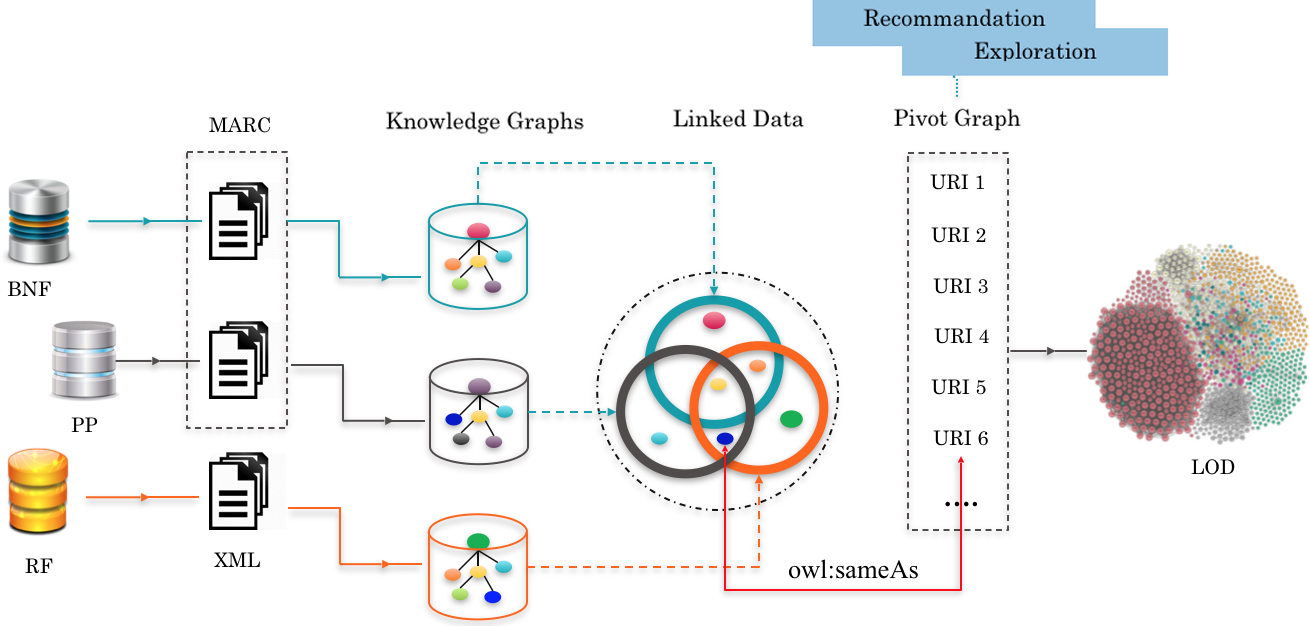
\includegraphics[width=11cm]{img/DRMS-WRKFL.png}
	\caption{The DOREMUS data lifecycle.}
	\label{fig:doremus}
%\end{figure}
\smallskip
%\begin{figure}
  \centering
  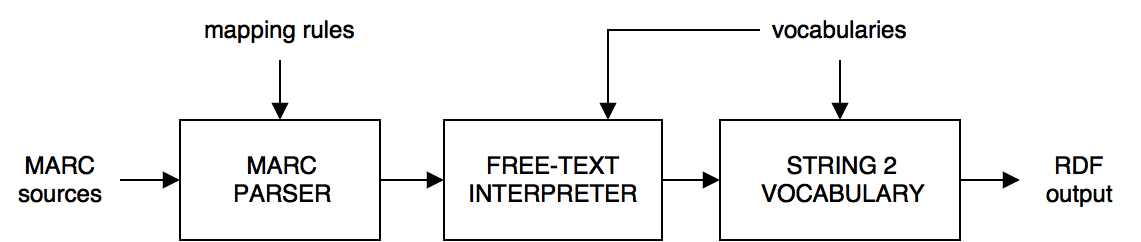
\includegraphics[width=8.5cm]{img/marc2rdf_schema.png}
  \caption{The application flow of \texttt{marc2rdf}.}
  \label{fig:marc2rdf}
\end{figure}

The converter is composed of different modules that work in succession (Fig.~\ref{fig:marc2rdf}). First, a \textit{file parser} reads the MARC file and makes the content accessible by field and subfield number. We implemented a converting module for both the INTERMARC and UNIMARC variants. Then, it builds the RDF graph reading the fields and assigning their content to the DOREMUS property suggested in the transfer rules. The \textit{free-text interpreter} extracts further information from the plain text fields, that includes editorial notes. This amounts to do a knowledge-aware parsing, since we search in the string exactly the information we want to instantiate from the model (i.e., the MoP from the casting notes, or the date and the publisher from the first publication note). The parsing is realized through empirically defined regular expressions, that are going to be supported by Named Entity Recognition techniques as future work. Finally, the \textit{string2vocabulary} component performs an automatic mapping of string literals to URIs coming from controlled vocabularies. All variants for a concept label are considered in order to deal with potential differences in naming terms. As additional feature, this component is able to recognize and correct noise that is present in the MARC file: this is the case of musical keys declared as genre, or fields for the opus number that actually contain a catalog number and vice-versa.

The {\tt marc2rdf} tool allows to reproduce deterministically the conversion process at any moment in time, providing the opportunity to seamlessly take into account possible updates of the ontology (e.g., the addition of a new property) and/or the data entries (a new record entering the catalog of one of the institutions), ensuring in that way the currentness and dynamics of the graphs. 

The works from Radio France, described in XML, are managed by an \textit{ad hoc} software that parses the input file, collects the required information, creates the RDF graph structure  and runs the \textit{string2vocabulary} module.% described previously.%\todo{I'm aware of the problem, but not providing a link to the converter might compromise the paper. Any ideas of solution?}

\subsection{Data Linking}
The three datasets that are currently subject to interlinking are highly heterogeneous: a given entity (e.g., a musical work) can be described quite differently across the three institutions. In addition to well-known data discrepancies such as lexical, semantic (polysemy, synonymy) and orthographic mismatches of string literals, the use of acronyms and abbreviations or differences in formats and types of numerical values, we have encountered several commonly occurring issues that are specific to our data. We outline some of them below.

%\begin{enumerate}
---~{\it Differences in coverage} and particularly lack of information in one of the graphs as compared to a richer description in another. In our case, the  works coming from RF are systematically described by a considerably smaller set of attributes, than those found in the catalogs of the BnF and the PP (see Table~\ref{tab:stats}). 

--- {\it Different depths in the graphs}, at which we find the value of interest---e.g., the birthplace of a composer can be directly assigned to the entity in one graph, or via a longer property chain in another. 

--- Presence of {\it comments in the form of free text} (given by the property {\tt ecrm:P3\_has\_note}) that are difficult to compare, as well as presence of {\it institution-specific resource identifiers} (bibliographical records ID's) given under the same property name across different datasets, although not comparable.% and therefore of little use for the linking task.

--- Presence of {\it blocks of  highly similar in their descriptions, but yet distinct instances} in each of the graphs---e.g., the set of all piano sonatas by Beethoven, differing from one another in only one or two property values, which makes their disambiguation difficult and is likely to produce false positives. 
%\end{enumerate}

In a first attempt to interconnect these graphs, we relied on state-of-the-art linking systems \cite{jentzsch2010silk,ngomo2011limes} that adopt a property-based philosophy where a set of attributes is selected in order to compare instances across two datasets based on (an aggregation of) similarity measures computed on their literal values. The results obtained proved to be not satisfactory.\footnote{Evaluation results of {\it Legato} on OAEI benchmarks can be found at \url{https://github.com/DOREMUS-ANR/legato/blob/master/Legato-Results.png}. Data and configuration files for SILK are available at \url{https://github.com/manoach/SILK-Evaluation}. Note that SILK is configured by using the best keys selected by the algorithm in \cite{achichiEST16}.}. Consequently, we develop our own linking tool, named \textit{Legato} \cite{achichi2017legato}---a generic data linking system motivated by the DOREMUS use-case scenario and data linking challenges. 

\begin{figure} 
\center
	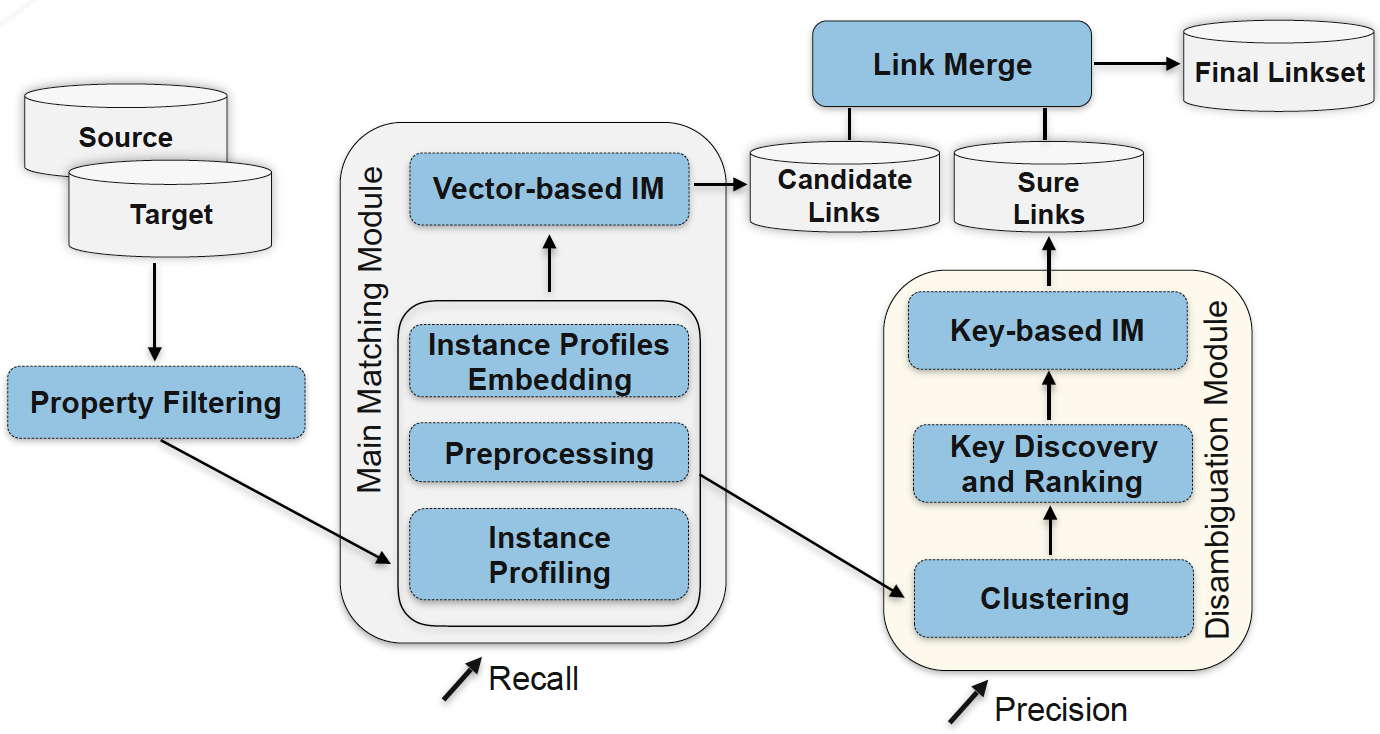
\includegraphics[width=9cm]{img/legato-wf-3.png}
    %\vspace{-0.2em}
	\caption{Processing pipeline of \textit{Legato}.}
	\label{fig:workflow}
	%\vspace{-2.5em}
\end{figure}

{\it Legato} is designed to match entities from highly heterogeneous graphs, effectively disambiguating highly similar yet distinct resources. Fig.~\ref{fig:workflow} shows the generic workflow of the system. The data cleaning module ensures to only keep properties that are comparable across the datasets (hence, comments in the form of free text, as well as institution-specific instance identifiers are removed). The instance profiling module represents instances by a subgraph corresponding to the union of the Concise Bounded Descriptions (CBD)\footnote{\url{https://www.w3.org/Submission/CBD/}} of each resource and its direct neighbors.  In that, contrarily to SILK or Limes, Legato (in its default version) does not compare property values, but considers all extractable literal values as a bag-of-words.  This representation addresses in its mechanism a number of data heterogeneities without requiring user input, in particular, the description differences and property depths discrepancies outlined above. The literals of these subgraphs are then used to project each instance in a vector space and the matching consists in comparing the resulting vectors. A deliberately low threshold is used for the vector similarity in order to ensure  high recall. Then, highly similar instances are grouped together by the help of a standard hierarchical clustering algorithm~\cite{RokachM05a}. An RDF key discovery \cite{SAKey} and a key ranking \cite{achichiEST16} algorithms are applied on each pair of similar clusters (identified by comparing cluster centroids) across the two graphs, in order to identify the set of properties that best allow to discriminate between the resources contained in each cluster. A new linkset (called ``sure links") results from this process and is then compared to the links produced at the matching step (called ``candidate links") in order to eliminate errors and increase precision, leading to the production of the final linkset. The outcome of {\it Legato} is presented in the EDOAL format,\footnote{\url{http://alignapi.gforge.inria.fr/edoal.html}}  allowing to keep track of the associated confidence scores, or as {\tt owl:sameAs} triples. We provide an open source implementation of the system together with a simple user interface (see Table \ref{tab:links} for a link).

Given our knowledge of the DOREMUS data, we have customized the linking process for the purposes of the project in two respects. (1) The linking workflow begins by searching for values of the composer name and catalog number properties, because the set of these two properties has been identified as a key by our experts. If values for these two properties are found for a given pair of instances, they are directly used for the comparison and {\it Legato} is executed on the remaining instances only. Note, however, that these properties do not have values for a very large number of works and in particular, no entry of {\tt itema3} has a catalog number (cf. Table~\ref{tab:stats}). (2) In order to speed-up the execution of {\it Legato}, we have partitioned the datasets per composer and linked pairs of subsets across two graphs that gather works by the same composer.

To evaluate {\it Legato}, we have constructed benchmarks of music works from the BnF and the PP, by asking the librarian experts to manually select pairs of identical resources from the their respective catalogs. We have ensured that our benchmarks are representative and provide a fair account of the heterogeneity issues outlined above. This results in the generation of two  benchmarks  that have been released by the Instance Matching track of OAEI 2016 and 2017 (cf. Table \ref{tab:links}). {\it Legato} has participated to the 2017 edition of the campaign, ranking first on the DOREMUS-FPT task. NjuLink surpasses {\it Legato} by 0.025 points (F1) on the DOREMUS-HT track, but performs worse by 0.044 points on the FPT track. Our data exhibits characteristics of the two, therefore we decided to go for {\it Legato}, in addition to the customizability argument given above.  
%(results are available on the OAEI 2017 website).

\subsection{ Link Validation and Pivot Graph Construction} \label{sec:pivot}
As a result of the pair-wise alignments of the three graphs, we end up with three sets of links. We exploit the topology of the connectivity of the entities of the three graphs in order to define subsets of links to provide to data experts for manual validation, aiming to ensure a final set of links of high quality. We identify four connectivity patterns, shown in Fig.~\ref{fig:cases}, according to which we classify the produced links to three categories: {\it certain links}, {\it invalid links} and {\it validation candidates}. The classification of a link as ``certain" depends both on its confidence value and on the connectivity pattern in which it falls. The certain links are retained and included in the pivot graph constructed from our data (see below). If a link is approved by an expert during the user validation process, its confidence value is set to 1, which automatically classifies it as ``certain", else it is declared as ``invalid". We consider the following link patterns.

\begin{figure} 
\center
	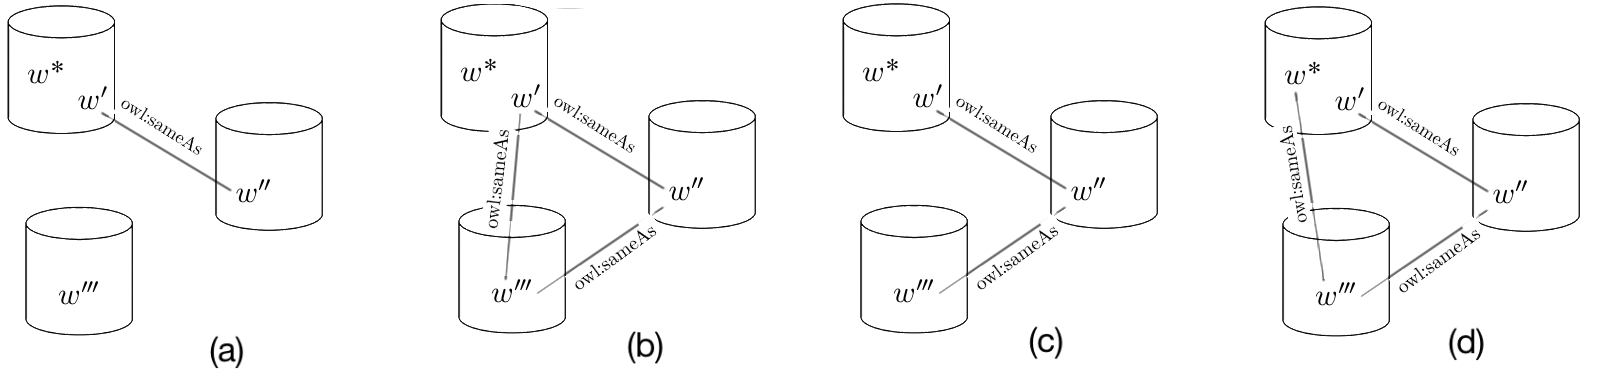
\includegraphics[width=12cm]{img/links-cases.png}
    %\vspace{-0.2em}
	\caption{Links across the three graphs: four connectivity patterns.}
	\label{fig:cases}
	%\vspace{-2.5em}
\end{figure}

%\begin{enumerate}
%\item 
(1) Single link. This is the case when two works are connected via an identity link across their corresponding graphs as a result of the automatic linking process (Fig.~\ref{fig:cases}(a)). According to the confidence value of the link, it is either classified as  certain, passed over to the experts for validation, or discarded.

(2) Triangle. This is the case when three works from the three graphs are linked via three {\tt owl:sameAs} relations. In this case, the three links are considered as certain and the expert is not solicited (Fig.~\ref{fig:cases}(b)).

(3) Missing link. This is the case when an instance $w'$ from one graph is linked to an instance $w''$ from the second graph, which in turn is linked to an instance $w'''$ from the third graph, but no link has been created between $w'''$ and $w'$ (Fig.~\ref{fig:cases}(c)). Instead of inferring that link, independently on the links confidence values, we pass the two link candidates $<w'$, {\tt owl:sameAs}, $w'' >$, $<w''$, {\tt owl:sameAs} $w'''>$ to the experts for validation. If the validation process results in classifying these two links as certain, the link $<w'''$, {\tt owl:sameAs}, $w'>$ is inferred and classified as certain. Note that the third link inference mechanism is activated only in case we have two certain links.

(4) Conflict. This is the case when an instance $w'$ from one graph is linked to an instance $w''$ from the second graph, which in turn is linked to an instance $w'''$ from the third graph, and $w'''$ is linked to an instance $w^*$ from the first graph, where $w' \neq w^*$  (Fig.~\ref{fig:cases}(d)). All three links are passed to the experts for validation. This necessarily leads to invalidating at least one of the three links, in which we fall into one of the three cases described above.
%\end{enumerate}

\begin{figure} 
\center
	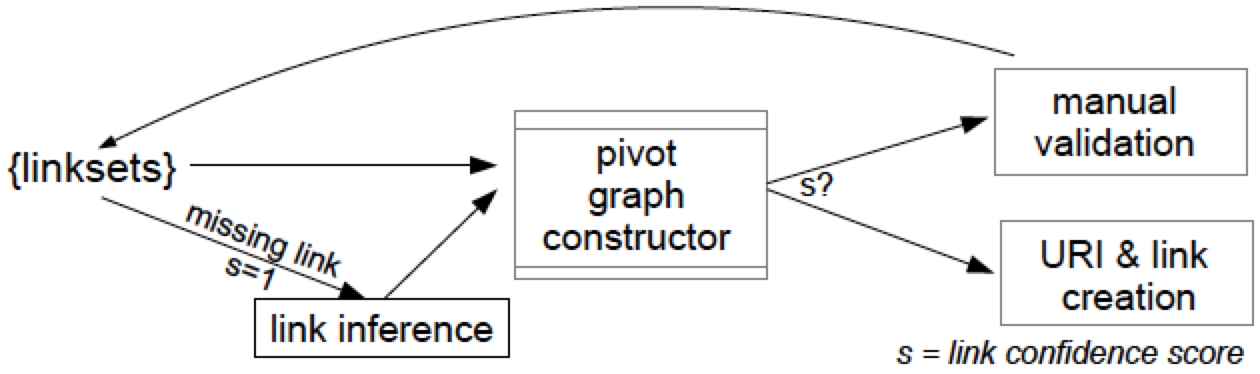
\includegraphics[width=7cm]{img/pivot-graph-2.png}
    %\vspace{-0.2em}
	\caption{Link validation and pivot graph construction workflow.}
	\label{fig:pivot}
\end{figure}

\vspace{-0.8cm}

\paragraph{Pivot Graph Construction.}
We construct a referential pivot graph of music works that is the mathematical union of the three sets of works from the three partner institutions. As an editorial decision, a novel URI is created for every entity in that graph, following the URI creation pattern described previously, together with a {\tt owl:sameAs} link to the URIs identifying this entity in each of the three input graphs (at least one such URI exists). For example, if a given expression is described in both the BnF and the PP graphs, the pivot graph will contain the following two triples: 
$<$PIVOT\_URI$>$ {\tt owl:sameAs} $<$BNF\_URI$>$, $<$PP\_URI$>$. If the work exists  in one single graph only (e.g., the  one of BnF), one single triple will be declared: $<$PIVOT\_URI$>$ {\tt owl:sameAs} $<$BNF\_URI$>$. To reconstitute these links, we rely on the linksets produced in the data linking phase and on the manual link validation task. As explained above, as a result of these processes, we end up with three sets of ``certain" links. Only links from that category will appear in the pivot graph. As Fig.~\ref{fig:pivot} shows, the process of pivot graph construction and that of the manual validation of links are tangled up in a single workflow. The code of the algorithm for (re-)generating the pivot graph is released as open source (cf. Table \ref{tab:links}).

Currently, the manual validation process is in progress. Therefore, the published pivot graph contains the links that have been identified automatically (i.e., corresponding to the patterns in Figs.~\ref{fig:cases}(a) and~\ref{fig:cases}(b)) by using the non-conservative thresholds of {\it Legato} tuned by the help of our benchmarks (0.2 for {\tt bnf}-{\tt philharmonie} and 0.5 for the other two pairs of datasets). The graph contains also the links of all unique works (those that have no matches found in any of the two other bases) to their original URIs. The results of the automatic link discovery process on the three bases together with the resulting pivot graph in its current shape are available at \url{https://github.com/DOREMUS-ANR/knowledge-base/tree/master/linked-data}. 

\paragraph{Links statistics.}

We have currently a total of 7495 links created automatically across the three graphs, among which we have 2520 links of type {\it single link}, 396 links of type {\it triangle}, 3378 links  of type {\it missing link} and 261 links  of type {\it conflict} (as labeled in Fig.~~\ref{fig:cases}), plus additional 940 links of type 1:many that are currently subject to post-processing. Updates in the datasets will not decrease the number of links since the source databases monotonically grow. 

%We have currently a total of 107684 links created automatically across the three graphs, among which we have 2887 links of type {\it single link}, 68886 links of type {\it triangle}, 2174 links  of type {\it missing link} and 293 links  of type {\it conflict} (as labeled above and illustrated in Fig.~~\ref{fig:cases}). Currently, this makes a total of 2467 links to validate manually, or $3\%$ of the total number of links produced. However, this number can potentially increase if more conservative thresholds are selected for the manual validation. Updates in the datasets will not decrease the number of links since the source databases monotonically grow. 

\section{The DOREMUS Resource In Use} \label{sec:use}
We proceed to discuss aspects related to the use of the resources, starting with their exploration and search.

{\texttt{Overture}: {\it an Exploratory Search Engine.}} We develop \textsc{Overture} (Ontology-driVen Exploration and Recommendation of mUsical REcords), a prototype of an exploratory search engine for DOREMUS data, available at \url{http://overture.doremus.org}. The application makes requests directly to the SPARQL endpoint and provides information in a web user interface (UI).

\begin{figure}[t]
 \centerline{
 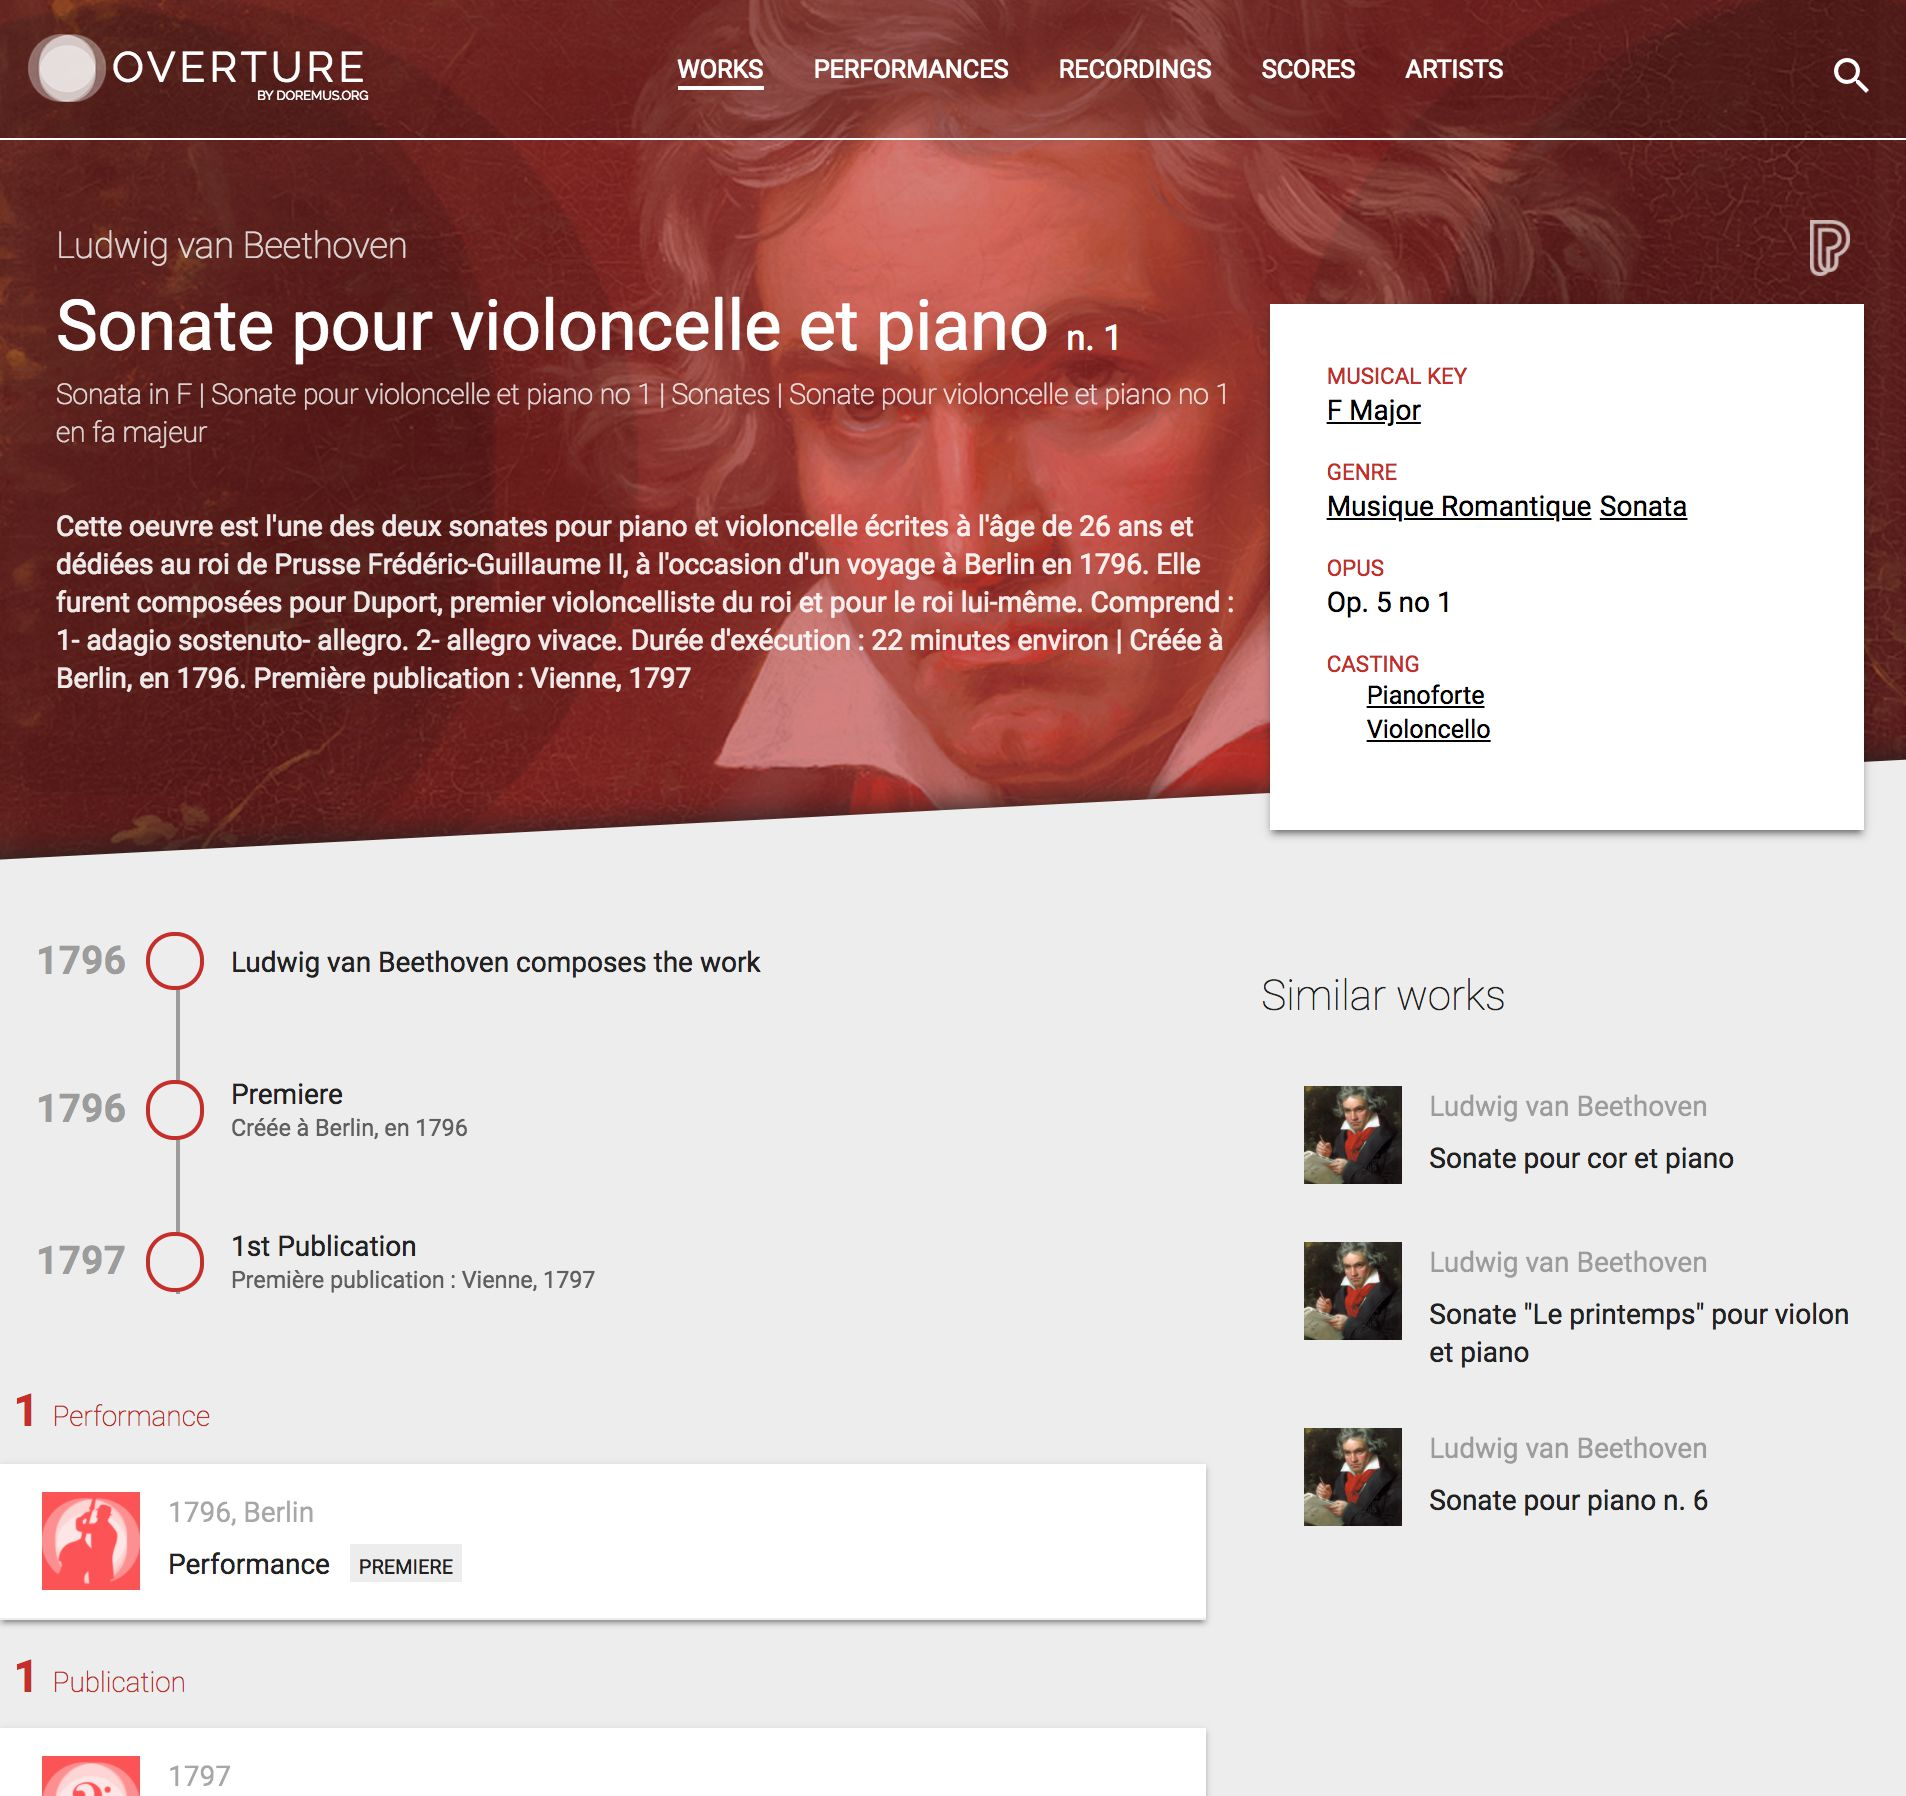
\includegraphics[width=10cm]{img/overture-sonata.jpg}}
 \caption{The detail of an expression in \textsc{Overture}}
 \label{fig:overture-detail}
\end{figure}

At the top of the UI, the menu bar allows the user to navigate between the main concepts of the DOREMUS model: expression, performance, score, recording, artist. Fig.~\ref{fig:overture-detail} represents Beethoven's \textit{Sonata for piano and cello n.1} as seen in \textsc{Overture}. Aside from the different versions of the title, the composer and a textual description, the page provides details on the information we have about the work, like the musical key, the genres, the intended MoP, the opus number. When these values come from a controlled vocabulary, a link is present in order to search for expressions that share the same value, for example, the same genre or the same musical key. A timeline shows the most important events in the story of the work (the composition, the premiere, the first publication). Other performances and publications can be represented below. 

The richness of the DOREMUS model offers to the end-user the chance to perform a detailed advanced search. All expressions (works) are searchable by facets, that include the title and the composer, but also keys, genres, detailed castings, making it possible to select very precise subsets of data, like all sonatas (genre) that involve a clarinet and a piano (MoPs). The hierarchical properties in the controlled vocabulary allow the smart retrieval not only of the entity that match exactly the chosen value (i.e. \textit{Strings}), but also any of its narrower concepts (i.e. \textit{violin}, \textit{cello}, etc.).

A {work-in-progress} recommendation system is also implemented in \texttt{Overture} in order to suggest to the final user different works to discover. The recommended works have similar properties to the current one, like the genre, the composer and the foreseen instruments. The recommendation is realized by computing knowledge graph embeddings using \textit{node2vec}~\cite{node2vec-kdd2016} on the DOREMUS knowledge graph and selecting the closer works using the euclidean distance~\cite{lisena2017artistsimilarity}.

Other client applications that also make use of the DOREMUS dataset include CityMus~\cite{lisena:iswc2017}, a mobile application that generates Spotify playlist composed of DOREMUS tracks based on the surrounding important buildings of a geo-localized user in a city. More precisely, interesting paths in the DBpedia knowledge base between POIs and composer are sought and shown to the end user in order to explain the recommendation. We also develop a chatbot that is capable of answering trivia questions in classical music.\footnote{\url{https://chatbot.doremus.org}}

\textit{Current Users and Impact.} The DOREMUS resource is currently used by librarians internally within each partner institution and across the three institutions, allowing for the fast retrieval of results for complex queries (see Table \ref{tab:links} for a link to examples). Thanks to the exploratory search engine, the DOREMUS data is open for access to a  wide community of musicians, music theorists, connoisseurs and amateurs, who do not need to have any technical expertise in order to query the RDF graphs. The controlled vocabularies and the DOREMUS ontology are also being endorsed by IFLA, as a de-facto standard for this community. The French National Library, per its conservation mission, guarantees that the DOREMUS resources will always be accessible and maintained.

Our goal is also to use the resources for both pedagogical and editorial purposes. The recommendation system that is currently under development will assist the creation of playlists for radios, allowing to group works together by very specific criteria, or to uncover rare works and provide insights about possible relations between composers, genres, events, etc.

We contribute to the semantic web community at large by providing open source implementations of novel and generic tools for data linking and fusion. We foster the adoption of semantic web technologies via the publication of numerous pedagogical materials, aiming to guide and encourage other cultural institutions to reuse the DOREMUS model and vocabularies and reproduce our data production framework (see Table \ref{tab:links}), as similar initiatives exist in other fields \cite{villazon2011methodological}.
\section{Related Work and Graphs} \label{sec:relwork}
There has been a significant effort in the last years to open and publish data from the field of cultural heritage \cite{dijkshoorn2014rijksmuseum}. An overview of related projects is given in \cite{marden2013linked}, where the authors provide an evaluation of the various initiatives with regard to the well-known five-stars open data  rating, applied to the cultural domain.%\footnote{\url{https://www.w3.org/DesignIssues/LinkedData.html}} 

Regarding the more specific problem of producing linked data out of library records, addressed by the DOREMUS project, a number of related initiatives have recently been introduced. We refer to the multiple contributions of the Europeana project,\footnote{\url{http://www.europeana.eu}}, unifying and making accessible the catalogs of  numerous libraries, museums and archives across Europe. One of the early efforts in that respect is made by the Library of congress,\footnote{\url{http://id.loc.gov}} which has become a dataset of reference in the field. In the same spirit, related projects include the German National Library linked data service,\footnote{\url{http://www.dnb.de/EN/lds}} the British National Bibliography Linked Data Platform,\footnote{\url{http://bnb.data.bl.uk/docs}} the open data project of the French National Library BnF\footnote{\url{http://data.bnf.fr}} or, more recently, the Virtual Library  Miguel de Cervantes project \cite{candela2017migration}.

In the majority of the cases, data comes  in a given MARC variant and has to be converted to RDF. In certain cases the migration process goes through an intermediate phase of translation to relational database \cite{candela2017migration}, or data is being directly converted to RDF based on the standards of bibliographical description, such as FRBR. DOREMUS follows this line of work by implementing its own expert-defined mappings-based conversion mechanism, enriching FRBRoo with more than 40 classes and 100 properties. The resulting (DOREMUS) model fills the important gap between library content description and music metadata. 

As compared to music-related datasets, we outline that the BBC open datasets have tracks only, the Dutch Library (part of Europeana) has only publications, CPDL\footnote{\url{https://www.cpdl.org/}} is specialized for chorus (with scores and midi), while DOREMUS is general and can glue these datasets. MusicBrainz \cite{musicbrainz}, one of the most popular knowledge bases about music metadata, started a few years ago its process of exposing its data as semantic triples through the platform LinkedBrainz \cite{linkedbrainz}. In contrast to DOREMUS, which follows a librarian structure, MusicBrainz follows a more commercial practice giving a central role to tracks, albums and artists (un-distinguishing the composer from the performer), at the expense of all the information connected to the work concept (genre, casting, key, etc).
\section{Conclusion and Future Work} \label{sec:conclusion}
We have presented the DOREMUS resource---a collection of linked RDF datasets representing the catalogs of music works of three major French cultural institutions. The construction of this resource implies the implementation of a processing pipeline that allows for the conversion of the original data to RDF following the DOREMUS ontology, the development, SKOS-ification and alignment of a number of music-specific vocabularies and the interlinking of the datasets, which results in the construction of a reference pivot graph of musical works shared by or unique to the three  institutions. This pipeline defines the data production paradigm of DOREMUS that is applicable to other music-library data---the described process is deterministic, extensible, reproducible and documented in numerous pedagogical materials published online. A number of tools acting at different layers of this pipeline have been introduced: the {\tt marc2rdf} data converter, the {\it Legato} data linking system, the web-interface for SKOS thesauri alignment and mapping validation and enrichment YAM++ {\it on line},  as well as the exploratory search engine \textsc{Overture}. We have relied on existing tools where appropriate (matching strings to URI), but the heterogeneity of the input data and the specificity of the librarian practices made this impossible in many cases. In terms of datasets, DOREMUS currently has published (1) three RDF graphs of musical works coming from the BnF, the Philharmonie de Paris and Radio France, (2) a pivot graph currently containing the certain links established automatically between the graphs of musical works, together with the results of the pairwise linking of these graphs, (3) expert curated benchmarks for evaluation of data linking systems, (4) a rich set of music-specific SKOS vocabularies together with their alignments.

We are currently in the process of applying the data conversion and linking workflow to two additional databases from Radio France. Natural Language Processing techniques are being included in the conversion process in order to parse the numerous free-text fields. \textsc{Overture} will soon host all the links between the interlinked works, giving access at the same time to the joined knowledge and to the different information provenances. We have developed a web interface to assist the process of manual validation of links reducing the human effort, which is currently being deployed online.  Alignments of our data to established datasets (in particular MusicBrainz) are currently being generated.

\section*{Acknowledgments}
This work has been partially supported by the French National Research Agency within the DOREMUS project, under grant ANR-14-CE24-0020.

\bibliography{bib}
\end{document}
